% p41-a-typical-element-would-look-like.tex
%
% Source: C. A. Gunter and D. S. Scott, "Semantic Domains", Handbook of
%   Theoretical Computer Science, Volume B, North Holland, 1990, pp. 633-674.
% Physical page: 41   Printed page: 40
% Section: 7.3, "Solving domain equations with projections."
% Introducing sentence (quoted verbatim from the paper):
%   "As the basis U_0 of our domain we take finite (non-empty) unions of half
%    open intervals [r,t) = {s in S | r <= s < t}. A typical element would look
%    like"
%
% The paper prints no caption and no figure number for this picture; the name
% above is taken from that sentence, per the r0039 naming rule.
%
% Why this file exists: this picture is a STREAM-4 FIND. `find-diagrams.py`
% requires a region at least 40 px tall at 100 dpi, and this one measures about
% 28 px tall at 100 dpi (physical page 41, y approximately 961-989). No row of
% analyses/diagram-candidates.2026-0808-10:32.orchestrator.log covers it: page
% 41 has exactly two rows, 165-262 and 620-773, and neither reaches y=961.
% It is the single false negative measured over all 44 pages.
%
% What it shows: a typical element of the basis U_0 -- the rational line S cut
% by consecutive half-open intervals, with the finitely many intervals that
% make up the element drawn as thick segments. Seven consecutive intervals are
% drawn; the second, fourth and sixth are thick, i.e. selected.
%
% Geometry: measured from a 300 dpi render of physical page 41 and mapped to cm
% by the linear transform x_cm = (x_px - 275)/118.11 (118.11 px = 1 cm at
% 300 dpi), so the interval widths, the wide gap at interval 3, and the small
% horizontal offset inside each ")[" delimiter pair are the paper's own. The
% delimiter glyphs measure about 78 px tall at 300 dpi, i.e. 0.66 cm; \Big
% delimiters at 10pt are the closest standard size.

\documentclass[border=6pt]{standalone}
\usepackage{tikz}
\begin{document}
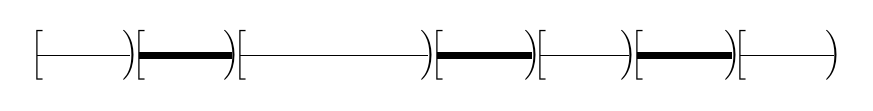
\begin{tikzpicture}[
  x=1cm, y=1cm,
  every node/.style={inner sep=1pt},
  open/.style={circle, draw, fill=white, minimum size=4pt, inner sep=0pt},
  solid/.style={circle, draw, fill=black, minimum size=5pt, inner sep=0pt},
  edge/.style={draw, line width=0.4pt},
  obj/.style={inner sep=3pt},
  arrow/.style={draw, line width=0.4pt, ->},
  darrow/.style={draw, line width=0.4pt, ->, dash pattern=on 4pt off 3pt}]

  % --- the seven consecutive half-open intervals, thin = not in the element ---
  \draw[line width=0.5pt] (0.000,0) -- (1.185,0);
  \draw[line width=0.5pt] (2.582,0) -- (4.970,0);
  \draw[line width=0.5pt] (6.393,0) -- (7.518,0);
  \draw[line width=0.5pt] (8.932,0) -- (10.118,0);

  % --- the three intervals that make up the element, drawn thick ---
  \draw[line width=2.5pt] (1.295,0) -- (2.480,0);
  \draw[line width=2.5pt] (5.080,0) -- (6.291,0);
  \draw[line width=2.5pt] (7.620,0) -- (8.831,0);

  % --- delimiters: "[" opens each interval, ")" closes it (half open) ---
  \node at (0.000,0)  {$\Big[$};
  \node at (1.185,0)  {$\Big)$};
  \node at (1.295,0)  {$\Big[$};
  \node at (2.480,0)  {$\Big)$};
  \node at (2.582,0)  {$\Big[$};
  \node at (4.970,0)  {$\Big)$};
  \node at (5.080,0)  {$\Big[$};
  \node at (6.291,0)  {$\Big)$};
  \node at (6.393,0)  {$\Big[$};
  \node at (7.518,0)  {$\Big)$};
  \node at (7.620,0)  {$\Big[$};
  \node at (8.831,0)  {$\Big)$};
  \node at (8.932,0)  {$\Big[$};
  \node at (10.118,0) {$\Big)$};

\end{tikzpicture}
\end{document}
